% This text is proprietary.
% It's a part of presentation made by myself.
% It may not used commercial.
% The noncommercial use such as private and study is free
% Nov. 2006
% Author: Sascha Frank 
% University Freiburg 
% www.informatik.uni-freiburg.de/~frank/
%
% additional usepackage{beamerthemeshadow} is used
%  
%  \beamersetuncovermixins{\opaqueness<1>{25}}{\opaqueness<2->{15}}
%  with this the elements which were coming soon were only hinted

\documentclass{beamer}
%\usepackage{beamerthemeshadow}
%\usetheme{Warsaw}
\usetheme{Amsterdam}
\usepackage[catalan]{babel}
\usepackage[utf8]{inputenc}
\usepackage{url}
\usepackage{eurosym}
\begin{document}
\title{Algorismes genètics aplicats a ciències de la vida}
\author{Raimon Grau Cuscó}
\date{\today}

\AtBeginSection[]
{
\begin{frame}
    \frametitle{Índex}
    \tableofcontents[currentsection]
\end{frame}
}

\frame{\titlepage} 

\frame{\frametitle{index}\tableofcontents} 

%\section{Motivació} % (fold)
%\label{sec:Motivacio}
%\begin{itemize}
	%\item hola
	%\item nanana ananan \ref{sec:Chiron}
	%\item adeu
%\end{itemize}
% section Motivació (end)


\section{Introducció} % (fold)

\begin{frame}
\frametitle{De què tracta aquest PFC?}
	\begin{columns}[c]
		\column{0.5\textwidth}
		\framebox{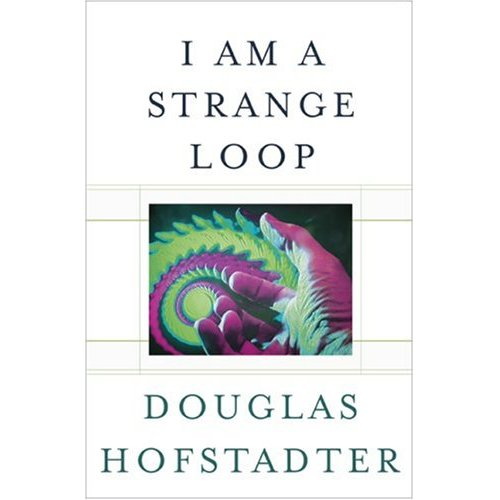
\includegraphics[height=0.9\textheight,width=0.9\textwidth]{images/StrangeLoop.jpg}}
		\column{0.5\textwidth}
		\begin{itemize}
			\item Tres projectes que utilitzen algorismes evolutius per a millorar processos en el
				disseny de nous farmacs
			\item Utilitzem tècniques apreses de com funciona la natura, per a després millorar la
				propia ``natura''.
			\item Oi que és un ``extrany bucle''?
		\end{itemize}
	\end{columns}
\end{frame}



\section{Algorismes evolutius} % (fold)
\label{sec:Algorismes evolutius}

\begin{frame}
	\frametitle{En la natura}
	\pause
	\framebox{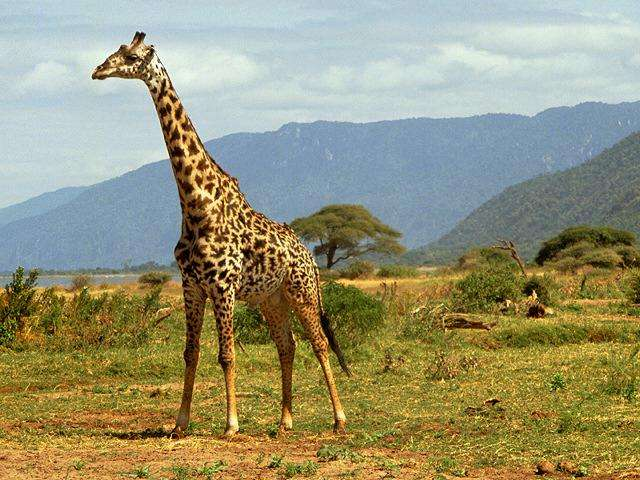
\includegraphics[height=0.9\textheight,width=0.9\textwidth]{images/jirafa11.jpg}}
\end{frame}
\begin{frame}
	\frametitle{Funcionament bàsic}
	\begin{columns}[c]
		\column{0.5\textwidth}
		\framebox{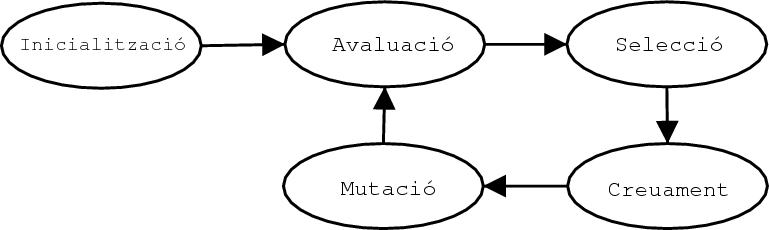
\includegraphics[height=0.4\textheight,width=0.9\textwidth]{images/ga.png}}
		\column{0.5\textwidth}
		\begin{itemize}
			\item Inicialització
			\item Avaluació
			\item Selecció
			\item Creuament
			\item Mutació
		\end{itemize}
	\end{columns}
\end{frame}

\begin{frame}
	\frametitle{Individu}
	\begin{block}{Què és?}
		Representació dels trets rellevants d'una possible solució al problema.
	 \end{block}
	\pause
	\begin{itemize}
		\item Ha de cumplir algunes condicions bàsiques per al problema (llargada, un cert crc,
			etc.) Durant tota la seva vida.
		\item No tots els trets del individu en l'entorn estan determinats pel seu codi genètic.
			(genotip vs fenotip)
	\end{itemize}
\end{frame}

\begin{frame}
	\frametitle{Inicialització}
	%\begin{columns}[c]
		%\column{0.5\textwidth}
		%\framebox{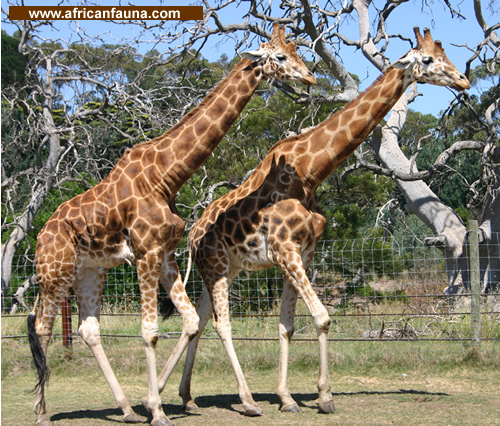
\includegraphics[height=0.7\textheight,width=0.9\textwidth]{images/giraffe-crossover.jpg}}
		%\column{0.5\textwidth}
		\begin{itemize}
			\item Primera població.
			\item Es generen els individus aleatòriament.
			\item Si hi ha restriccions, s'han de complir.
		\end{itemize}
	%\end{columns}
\end{frame}

\begin{frame}
	\frametitle{Fitness: Com de bo és un individu? (Avaluació)} 
	\begin{itemize}
		\item És el propi problema.  Fa el paper de l'entorn en el que està
		l'individu.
		\item Cada individu l'enfrontem a la funció de fitness.
		\item Retorna un valor (numèric) que ens permet comparar la bondat dels
		individus entre ells
	\end{itemize}
	\pause
	\begin{alertblock}{Compte!}
		Aquesta funció s'executa moltes vegades s'ha d'anar amb compte amb el
		cost
	\end{alertblock}
\end{frame}

\begin{frame}
	\frametitle{Selecció}
		\begin{block}{Els escollits}
			Quins individus es reproduiràn, per passar el seu codi genètic a la següent
			generació?
		\end{block}
		\pause
		\begin{itemize}
			\item Accedeixen a reproduir-se un percentatge molt alt de la
			població.
			\item Diferents tipus de mecanismes de selecció.
			\item Un o altre mecanisme pot provocar diferències molt grans en
			els resultats del algorisme.
			\item Es el responsable de la pressió evolutiva i la convergència
			prematura.
		\end{itemize}
		%\begin{exampleblock}
		%\end{exampleblock}
\end{frame}

%XXX chicha sobre seleccio  Ruleta i torneig

\begin{frame}
	\frametitle{Creuament}
	\begin{block}
		Mecanismes pels cuals creem descendència a partir de 2 individus
		existents.
	\end{block}
		\begin{itemize}
			\item Varia en funció del problema. %\verbatim{1100110011  001100110011}
			\item S'ha de ``pensar'' en el tipus de problema, i decidir
			\item Hi ha creuaments específics per algun tipus de problema (TSP).
		\end{itemize}
\end{frame}

%epistàcia   1p, 2p, mantenint posicions, creuant, etc..

\begin{frame}
	\frametitle{Mutació}
		\begin{itemize}
			\item Una vegada fet el creuament, un percentatge molt petit de la nova
			població pateix mutacions en algun dels seus gens.
			\item Les mutacions provoquen diferències dràstiques respecte el
			cromosoma no mutat.
			\item Va en contra de la convergència de la població.
		\end{itemize}
\end{frame}


\begin{frame}
\frametitle{Estat de l'art}
\begin{itemize}
\item Des que Holland publica sobre algorismes genètics, s'han utilitzat cada
cop en més àmbits
\item La gran potència de càlcul actual permet la seva utilització per tot tipus
de problemes
\pause
\item Als inicis s'utilitzava lisp.
\item Actualment existeixen llibreries en gairebé tots els llenguatges.
\item En els últims 10 anys, s'han buscat maneres de paralelitzar els algorismes
genètics.
\end{itemize}
\end{frame}

%\begin{frame}
	%\frametitle{Creuament}
	%\begin{columns}[c]
		%\column{0.5\textwidth}
		%\framebox{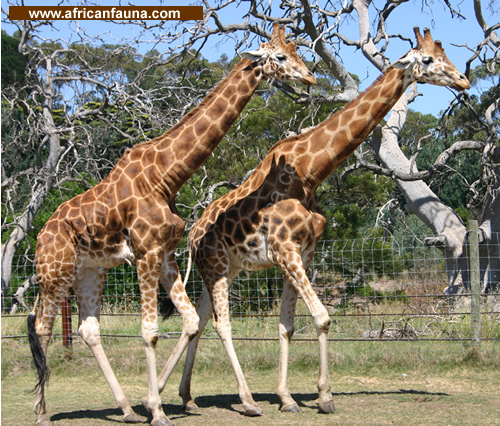
\includegraphics[height=0.7\textheight,width=0.9\textwidth]{images/giraffe-crossover.jpg}}
		%\column{0.5\textwidth}
		%\begin{itemize}
			%\item 
				%\pause
			%\item matat
		%\end{itemize}
	%\end{columns}
%\end{frame}
%% section Algorismes evolutius (end)

\section{Pholus} % (fold)
\label{sec:Pholus}

\begin{frame}
	\frametitle{Introducció}
	Per detectar similituds entre molècules volem detectar quins indicadors són
	més rellevants, i com ho són. 
	\pause
	\begin{itemize}
		\item Enfrontem un conjunt petit de molècules actives amb una llista llarga de molècules,
			que contenen aquestes actives, junt amb inactives.
		\item Cada molècula té 22 descriptors que la defineixen.
		\item Busquem 22 ponderacions que ordenin la llista completa posant les actives en les
			primeres posicions
	\end{itemize}
\end{frame}

\begin{frame}
\frametitle{Aproximació}
	\begin{itemize}
		\item Creem un Algorisme genètic que busca ponderacions que ordenin les actives al principi.
		\item L'usuari proporciona una llista d'actives i una llista amb totes les molècules, junt
			amb els descriptors
	\end{itemize}
\end{frame}

\begin{frame}
\frametitle{Funcionament general}
	%\begin{itemize}
	%\item 
	%\end{itemize}
\end{frame}

\begin{frame}
	\frametitle{Individu}
	Els individus són vectors de 22 números en coma flotant, entre -1 i 1, que descriuen.
\end{frame}

\begin{frame}
	\frametitle{Avaluació}
	\begin{block}{}
		Donada una ponderació per a cadascun dels 22 descriptors, la llista d'actives, i la llista
		completa, dona un valor de bondat de la ordenació.
	\end{block}
	\pause
	\begin{itemize}
		\item Utilitzem Bedroc com a mesura de bondat d'ordenació.
		\item Una molècula pot estar vàries vegades en la llista, donat que hi ha diferents
			conformacions en la natura.  En evaluar el Bedroc ens quedem amb la millor conformació
			de cada molècula.
	\end{itemize}
\end{frame}

%\begin{frame}
	%\frametitle{BEDROC??}
%\end{frame}

\begin{frame}
\frametitle{Operadors}

 % theme=Berlin;caption=Operadors Pholus
 % Operador & Valor
 % Inicialització & aleatòria [-1 , +1]
 % Selecció & 0.2
 % Creuament & 0.4
 % Mutació & 0.7

\begin{table}
\centering
\begin{tabular}{|l|l|}
\hline
\multicolumn{1}{|c|}{\textbf{Operador }} & \multicolumn{1}{c|}{\textbf{ Valor}} \\
\hline
\hline
Inicialització & aleatòria [-1 , +1] \\
Selecció       & Torneig(2) amb elitisme  \\
Creuament       &  unipunt        \\
Mutació        &   0.1                  \\
\hline
\end{tabular}
\caption{Operadors Pholus}
\end{table}

\end{frame}

\begin{frame}
\frametitle{Implementació}
\begin{tabular}[h!]{|c|c|}
	AE                                         & eodev (c++)                \\ 
	Interfície & Perl    \\ 
\end{tabular}
\end{frame}

\begin{frame}
	\frametitle{Testeig}
	\begin{block}{Sobreentrenament}
		Si entrenem un algorisme evolutiu per un conjunt molt petit de dades, el Algorisme pot
		sobreentrenar la solució per al nostre conjunt de test.
	\end{block}
	\begin{itemize}
		\item Separem les nostres dades en 3 conjunts: Train, Test i validació.
		\item Mirant els resultats obtinguts respecte el conjunt de test i validació podem saber si
			s'ha sobreentrenat.
	\end{itemize}
\end{frame}

% section Pholus (end)

\section{Chiron} % (fold)
\label{sec:Chiron}
% section Chiron (end)
\begin{frame}
	\frametitle{Química combinatòria}
	\begin{itemize}
		\item Esquelet que presenta certa activitat
		\item Hi ha punts on podem unir-hi seqüències d'atoms
		\item Aquestes seqüències estan ja definides quines poden haver-hi en cada punt d'unió
	\end{itemize}
	\pause
	\begin{block}{Objectiu}
		Volem trobar la combinació de substituients que maximitzi la bondat del esquelet
	\end{block}
\end{frame}

\begin{frame}
	\frametitle{Aproximació}
	Construir un programa que permeti trobar la combinació de substituients que
	maximitza la seva activitat.

	El procés ha de ser avaluat sintetitzant cada molècula.

	Utilitzem algorismes evolutius per a optimitzar el número d'avaluacions, ja
	que és un procés molt car.
\end{frame}

\begin{frame}
	\frametitle{Abstracció}
	\begin{itemize}
	\item Aprofitem creuaments i mutacions, però no tenim funció d'avaluació.
	\pause
	\item Podem abstraure el problema i convertir Chiron en un framework
	d'algorismes genètics.
	\end{itemize}
\end{frame}

%explicar chiron en general
\begin{frame}
\frametitle{Funcionament general}
\begin{itemize}
\item Introducció de les característiques del problema (numero de substituients,
i possibles substituients en cada posició)
\item Generació de població inicial
\item Introducció dels fitness de cada individu
\item següent iteració\ldots
\end{itemize}
\pause
L'usuari pot decidir si l'experiment ha de recordar els fitness dels elements ja
evaluats, i no mostrar els individus repetits.
\end{frame}

\begin{frame}
\frametitle{Operadors utilitzats}

 % theme=Berlin;caption=Operadors Chiron
 % Operador & Valor
 % Inicialització & aleatòria
 % Selecció & 0.2
 % Creuament & 0.4
 % Mutació & 0.7

\begin{table}
\centering
\begin{tabular}{|l|l|}
\hline
\multicolumn{1}{|c|}{\textbf{Operador }} & \multicolumn{1}{c|}{\textbf{ Valor}} \\
\hline
\hline
Inicialització & aleatòria \\
Selecció       &  Torneig(2) amb elitisme       \\
Creuament       & unipunt  \\
Mutació        & 0.5        \\
\hline
\end{tabular}
\caption{Operadors Chiron}
\end{table}
\end{frame}

\begin{frame}
\frametitle{Problemes d'inicialització}
En el nostre problema real, hi ha molt pocs individus que tinguin un fitness !=
0.
\pause
\begin{alertblock}{Alerta!}
Si en la primera generació tots els individus tenen el mateix fitness, la segona
generació (creada a partir de la primera) tindrà bàsicament elements de la
primera generació, provocant convergència prematura.
\end{alertblock}
\pause
\begin{exampleblock}{Solució}
En la primera generació, ens assegurem que no tots tinguin igual fitness.  Si és
així, creem una població nova aleatòria, per abarcar tot l'espai de búsqueda
\end{exampleblock}
\end{frame}

\begin{frame}
\frametitle{Tecnologies utilitzades}
\begin{tabular}[h!]{|c|c|}
AE & eodev (c++) \\
BBDD & Mysql + DBIX::Class (Perl) \\
WebService & SOAP \\
Enllaç $AE\rightarrow BBDD\rightarrow WS$ & Perl + Template Toolkit\\
Client SOAP & PHP , Perl , C++ \\
\end{tabular}
\end{frame}

\begin{frame}
	\frametitle{API}
	\begin{itemize}
		\item \textbf{newExp} (\$user, \$name, \$numAleles, \$popSize, \$cached , \$bounds)
		\item \textbf{removeExp} (\$idExp)
		\item \textbf{listExp} (\$userName)
		\item \textbf{setFitness} (\$idInd, \$f)
		\item \textbf{nextIteration} (\$idExp)
		\item \textbf{listIndividualsByExp} (\$idExp)
		\item \textbf{wipe}
	\end{itemize}
\end{frame}

\begin{frame}
	\frametitle{Resultats}
	\begin{columns}[c]
		\column{0.5\textwidth}
		\framebox{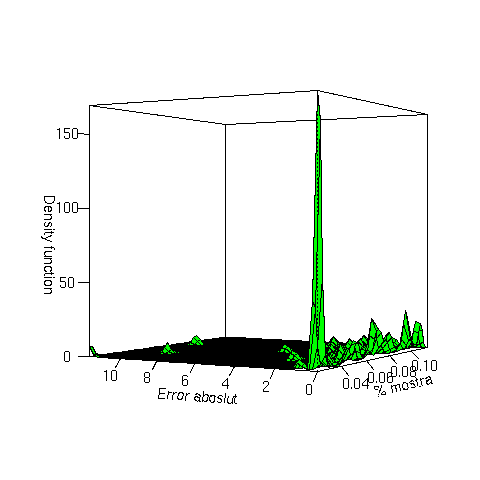
\includegraphics[height=0.7\textheight,width=0.9\textwidth]{images/rgrau1.png}}
		\column{0.5\textwidth}
		Chiron s'ha testejat en 3 problemes reals, amb un espai de cerca de més de 15000
		possibilitats, i en un 40\% ha trobat la millor combinació explorant només un
		12\% de les possibilitats.
	\end{columns}
\end{frame}

\section{GEP} % (fold)
\label{sec:GEP}
% section GEP (end)

%\begin{frame}
	%\frametitle{Introducció}
%\end{frame}

\begin{frame}
	\frametitle{Genetic Expression programming}
	\begin{center}
		\framebox{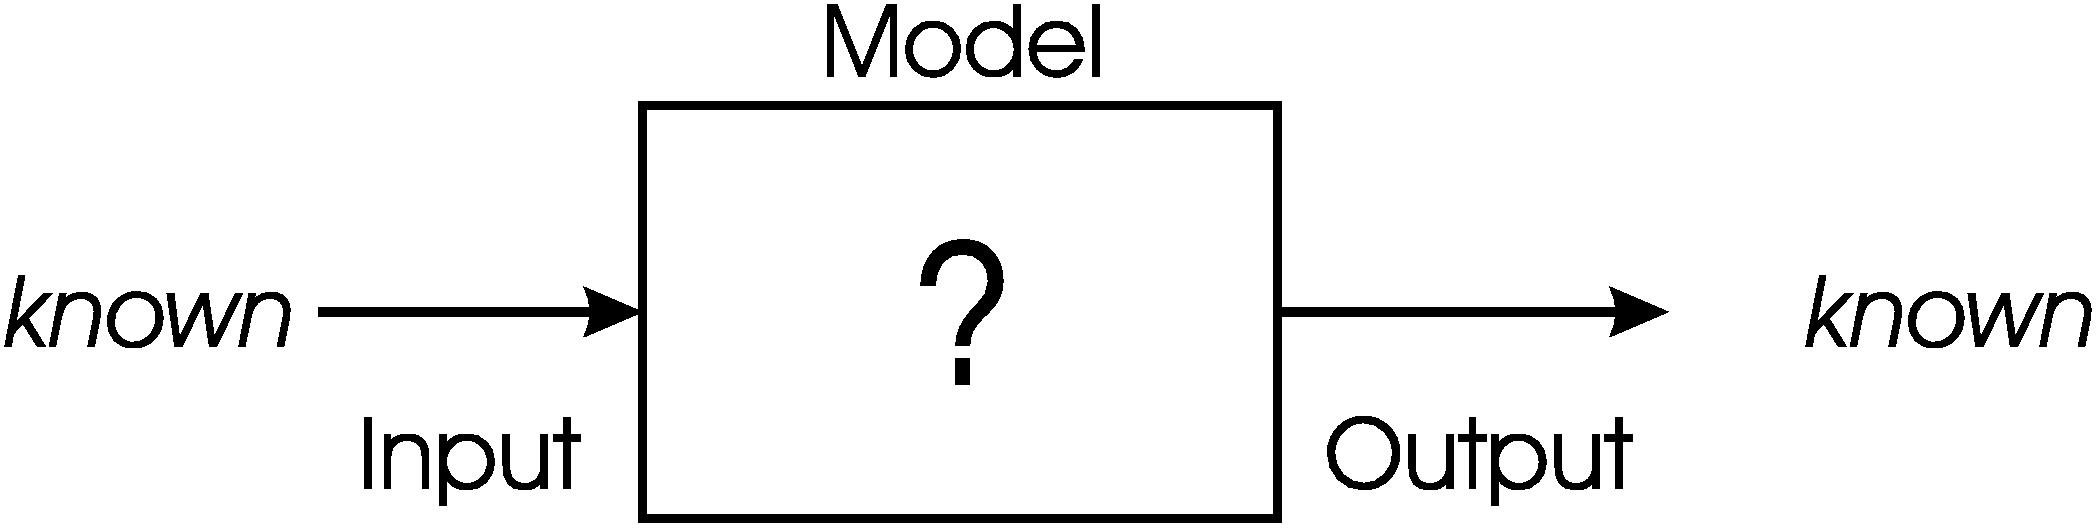
\includegraphics[scale=0.4]{images/1-5.jpg}}
	\end{center}
	\begin{itemize}
		\item Millora sobre la programació genètica (2001)
		\item Busquem optimitzar un procés i no pas la entrada d'un procés
		\item Els individus són processos, que hem d'optimitzar per tal que donada una entrada,
			evaluin a una sortida que volem.
	\end{itemize}
	\pause
	\begin{block}{Objectiu}
		Volem trobar fórmules matemàtiques a partir de angles de rotació en els
		enllaços d'una molècula i els seus volums.
	\end{block}
\end{frame}

\begin{frame}
	\frametitle{Funcionament general}
	\begin{itemize}
		\item Els individus són fórmules matemàtiques
		\item A diferència de en la programació genètica, podem fer creuaments i
		mutacions a nivell de genotip.
		\item A part d'això, funcionen igual que els algorismes genètics que ja
		hem vist.
	\end{itemize}
\end{frame}

\begin{frame}
	\frametitle{Notació Karva}
	\begin{columns}[c]
		\column{0.5\textwidth}
		+/*abcd

		\framebox{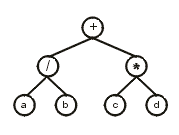
\includegraphics[height=0.5\textheight,width=0.7\textwidth]{images/pt01.png}}

		\column{0.5\textwidth}
		\begin{itemize}
			\item 2 tipus de nodes: Terminals (aritat 0) i operadors (aritat
			$>0$)
			\item Separem el nostre cromosoma en 2 parts, el \emph{head}, que
			conté operadors i terminals i el \emph{tail}, que només conté
			terminals.
		\end{itemize}
		\begin{block}{Els arbres sempre seran sintàcticament correctes si:}
			$$ t =  h (n-1) + 1 $$
			On n és la aritat màxima que podem trobar en un operador
		\end{block}
	\end{columns}
\end{frame}

\begin{frame}
	\frametitle{Notació Karva II}
	\begin{itemize}
		\item Composem un individu a partir de molts gens.
		\item Un dels sub-arbres no té referències a terminals sinó als altres sub-arbres
	\end{itemize}
\end{frame}

\begin{frame}
	\frametitle{Avaluació}
	\begin{itemize}
		\item Per avaluar un individu, el convertim a l'arbre d'expressió corresponent, i
			l'``executem'' amb els mostrejos que tenim.
		\item Comparem el resultat obtingut amb l'esperat.
		\item La diferència entre els resultats esperats i els obtinguts és el fitness (minimitzem)
	\end{itemize}
\end{frame}

\begin{frame}
	\frametitle{Operadors}
	Tots els operadors poden ser iguals que en els algorismes genètics clàssics
	gràcies a la notació Karva.
	\pause
	\begin{itemize}
		\item Inicialització: Aleatòria, respectant head i tail.
		\item Creuament: Unipunt, bipunt, creuament de subarbres.
		\item Mutació: Translació de zones i intercanvi de gens.
	\end{itemize}
\end{frame}

\begin{frame}
	\frametitle{Resultats}
	Hem tingut èxit amb funcions polinòmiques relativament complexes
	$$ f(x) = x^6 -2x^4 + x^2 $$
	\pause
	NO hem tingut èxit amb funcions periòdiques, que era l'objectiu on voliem
	aplicar GEP.

	$$ :( $$
\end{frame}

\section{Planificació i costos} % (fold)
\label{sec:Planificacio i costos}

\begin{frame}
	\frametitle{Pholus}
		\framebox{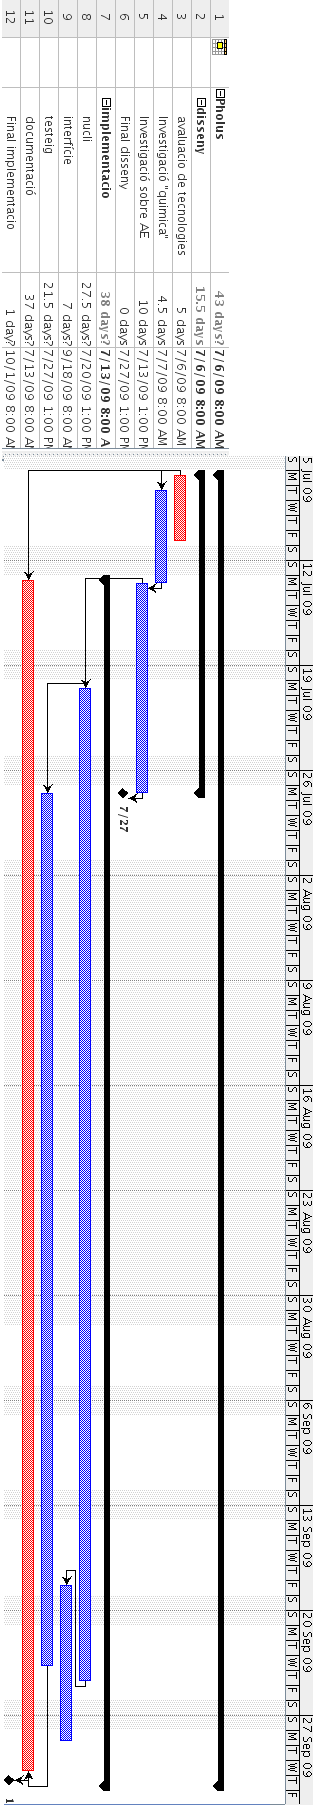
\includegraphics[height=0.5\textheight,width=1\textwidth]{../pholus/pholus-gantt.png}}
\end{frame}

\begin{frame}
	\frametitle{Chiron}
		\framebox{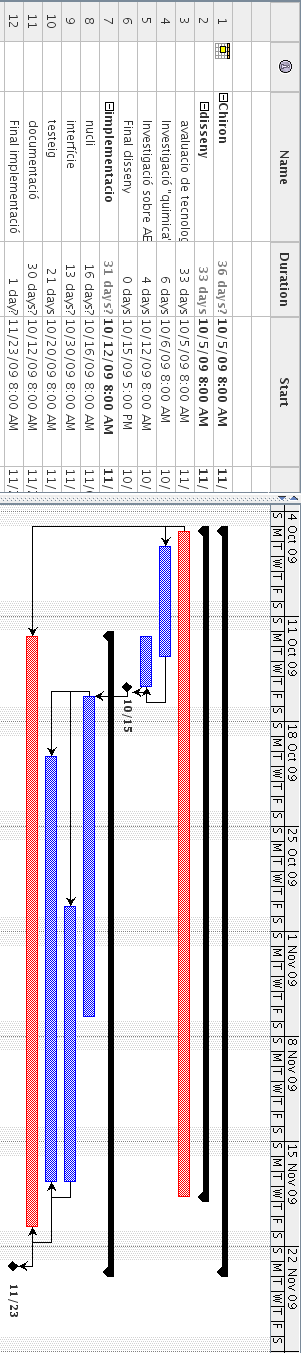
\includegraphics[height=0.5\textheight,width=1\textwidth]{../chiron/chiron-gantt.png}}
\end{frame}

\begin{frame}
	\frametitle{GEP}
		\framebox{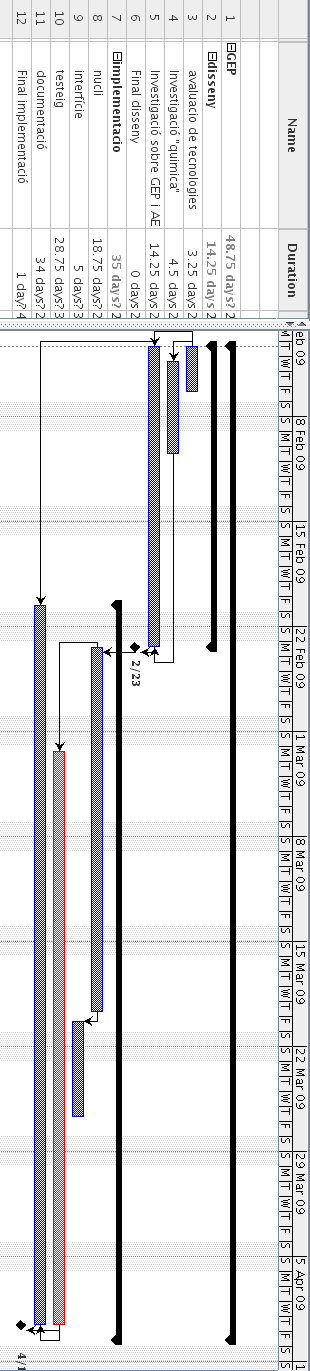
\includegraphics[height=0.5\textheight,width=1\textwidth]{../gep-gantt.png}}
\end{frame}

\begin{frame}
	\frametitle{Memòria}
\end{frame}

\begin{frame}
	\frametitle{Costos}
	Pholus = \EUR{3500} 

	Chiron = \EUR{3000} 

	GEP  = \EUR{3000} 

	Total = \EUR{9500}
\end{frame}

% section Planificació i costos (end)

\section{Conclusions} % (fold)
\label{sec:Conclusions}

\begin{frame}
	\begin{itemize}
		\item Aplicació d'algorismes genètics a problemes reals
		\item La intercomunicació entre processos és vital per a fer programes reutilitzables
		\item Utilització de moltes tecnologies diferents (MySql,Perl,eodev,SOAP,Template
			Toolkit,mercurial,git)
		\item Treballant amb tecnologies noves, la manca de literatura pot ser un impediment a
			l'hora d'aconseguir els objectius.
	\end{itemize}
\end{frame}

\begin{frame}
	\frametitle{FI}
	Gràcies per la seva atenció.

	Preguntes?

	\begin{center}
	\framebox{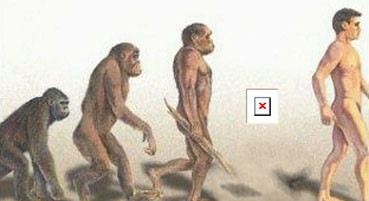
\includegraphics[height=0.5\textheight,width=0.6\textwidth]{images/mlink.jpg}}
	\end{center}

	Podeu trobar la memòria a \url{http://github.com/kidd/pfc}

\end{frame}
% subsubsection hola matat (end)

% section Conclusions (end)

\end{document}
